\documentclass[11pt]{article}

\usepackage[margin=1in]{geometry}
\usepackage[hidelinks]{hyperref}
\usepackage{enumitem}
\usepackage{booktabs}
\usepackage{tabularx}
\usepackage{tikz}
\usetikzlibrary{arrows.meta}

\title{Luphra MicroCover\\
\large Faruk Catak}
\author{}
\date{\today}

\begin{document}
\maketitle
\tableofcontents
\newpage

\section{Context and Scope}

Luphra MicroCover is a hackathon demonstration of per-action insurance for
autonomous AI agents. An agent requests coverage before performing an economic
action, receives a quote, pays a small premium through x402 on Algorand, and
receives a coverage receipt.

The initial demonstration covers one scenario: a procurement agent buying API
credits from a new vendor. It is intended to prove the payment and coverage
workflow, not to provide a production insurance product.

\subsection{Problem}

AI agents can spend money, call tools, communicate with third parties, and make
decisions on behalf of users. Existing controls generally allow or deny an
action. They do not attach dynamically priced financial protection to an
individual action.

Traditional insurance premiums are also poorly matched to agent activity. The
risk can vary with the transaction amount, vendor, requested action, user
policy, model confidence, and execution context.

\subsection{Current Status}

The repository contains a minimal Python FastAPI resource server. The
\texttt{/coverage} endpoint is protected by x402 middleware and advertises an
Algorand TestNet USDC payment. A paying agent client, dynamic quote service,
and coverage receipt are not yet implemented.

\section{Goals and Non-Goals}

\subsection{Goals}

\begin{itemize}[leftmargin=*]
  \item Demonstrate an HTTP 402 payment flow on Algorand TestNet.
  \item Let a Python agent automatically pay for a protected API resource.
  \item Generate a simple quote for an agent action.
  \item Return a coverage receipt containing the quote and settlement reference.
  \item Keep the implementation small enough to explain and demonstrate live.
\end{itemize}

\subsection{Non-Goals}

\begin{itemize}[leftmargin=*]
  \item Production insurance underwriting, licensing, or claims administration.
  \item MainNet payments or real customer funds.
  \item Building a custom facilitator or operating an Algorand node.
  \item Deploying an AVM smart contract.
  \item Supporting EVM, Solana, subscriptions, or fiat checkout.
  \item Building a complete customer dashboard.
\end{itemize}

\section{Design Overview}

\subsection{x402 Payment Sequence}

\begin{figure}[ht]
\centering
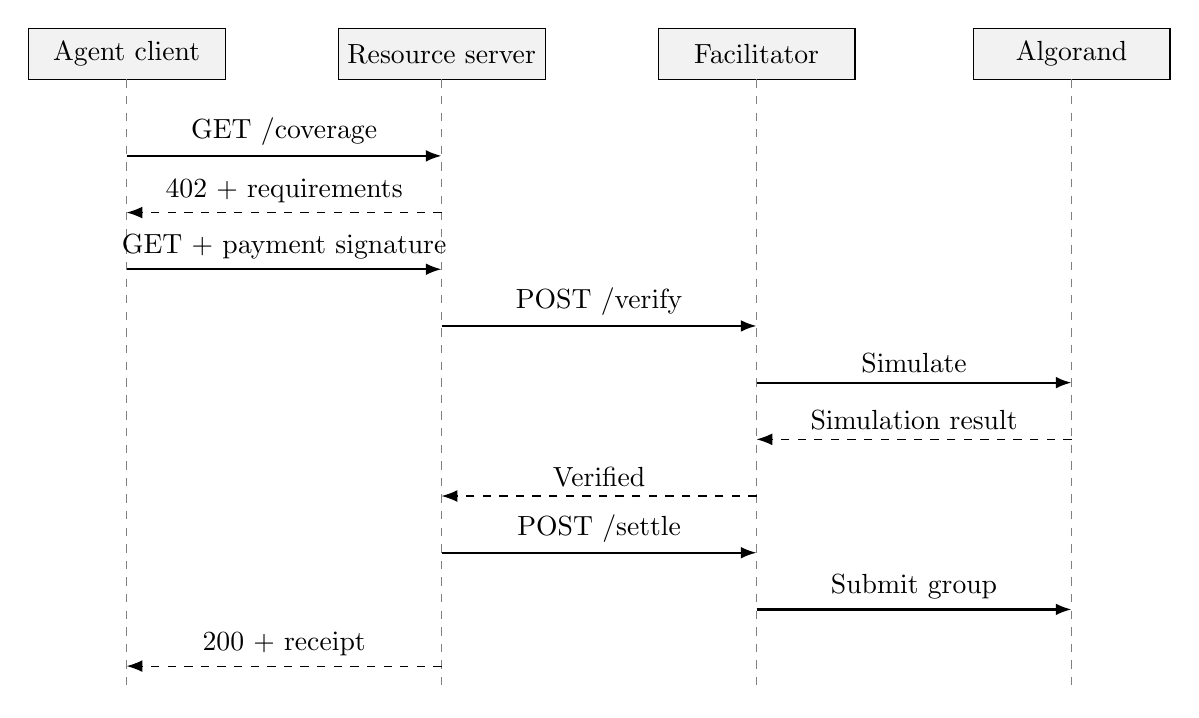
\begin{tikzpicture}[
  x=1cm,y=0.72cm,
  participant/.style={draw,fill=gray!10,minimum width=2.5cm,minimum height=0.65cm},
  lifeline/.style={gray,dashed},
  message/.style={-{Latex[length=2mm]},thick},
  return/.style={-{Latex[length=2mm]},dashed}
]
  \node[participant] at (0,0) {Agent client};
  \node[participant] at (4,0) {Resource server};
  \node[participant] at (8,0) {Facilitator};
  \node[participant] at (12,0) {Algorand};
  \foreach \x in {0,4,8,12} \draw[lifeline] (\x,-0.45) -- (\x,-11.2);
  \draw[message] (0,-1.8) -- node[above]{GET /coverage} (4,-1.8);
  \draw[return] (4,-2.8) -- node[above]{402 + requirements} (0,-2.8);
  \draw[message] (0,-3.8) -- node[above]{GET + payment signature} (4,-3.8);
  \draw[message] (4,-4.8) -- node[above]{POST /verify} (8,-4.8);
  \draw[message] (8,-5.8) -- node[above]{Simulate} (12,-5.8);
  \draw[return] (12,-6.8) -- node[above]{Simulation result} (8,-6.8);
  \draw[return] (8,-7.8) -- node[above]{Verified} (4,-7.8);
  \draw[message] (4,-8.8) -- node[above]{POST /settle} (8,-8.8);
  \draw[message] (8,-9.8) -- node[above]{Submit group} (12,-9.8);
  \draw[return] (4,-10.8) -- node[above]{200 + receipt} (0,-10.8);
\end{tikzpicture}
\caption{The HTTP 402 verification and settlement sequence.}
\end{figure}

\subsection{Component Responsibilities}

\begin{tabularx}{\textwidth}{@{}lX@{}}
\toprule
\textbf{Component} & \textbf{Responsibility} \\
\midrule
Agent client &
Requests coverage, holds the paying account, signs payment transactions, and
retries a request after receiving HTTP 402. \\
Luphra resource server &
Publishes payment requirements, returns quotes and coverage receipts, and
delegates verification and settlement. \\
Hosted facilitator &
Validates the proposed payment, optionally supplies fee abstraction, submits
the transaction group, and reports settlement. \\
Algorand TestNet &
Records and finalizes the USDC payment. \\
\bottomrule
\end{tabularx}

\section{Detailed Design}

\subsection{Technical Stack}

\subsubsection{Platforms and Services}

\begin{tabularx}{\textwidth}{@{}lX@{}}
\toprule
\textbf{Technology} & \textbf{Use} \\
\midrule
Python 3.12 & Application language. \\
FastAPI & HTTP resource server. \\
GoPlausible facilitator & Hosted verification and settlement service. \\
Algorand TestNet USDC & Demonstration payment asset. \\
LORA & Transaction inspection and debugging. \\
\bottomrule
\end{tabularx}

\subsubsection{Python Packages}

\begin{tabularx}{\textwidth}{@{}lX@{}}
\toprule
\textbf{Package} & \textbf{Reason} \\
\midrule
\texttt{x402-avm[fastapi,avm,httpx]} &
Provides the FastAPI payment middleware, Algorand payment mechanism, and
automatic paying client integration. \\
\texttt{fastapi} &
Defines the resource-server routes and HTTP responses. \\
\texttt{uvicorn} &
Runs the FastAPI application as an ASGI server. \\
\texttt{httpx} &
Provides asynchronous HTTP requests for the paying agent client. \\
\texttt{py-algorand-sdk} &
Derives Algorand addresses and signs the agent's payment transactions. It is
installed by the AVM extra. \\
\texttt{python-dotenv} &
Loads local configuration from the uncommitted \texttt{.env} file. \\
\texttt{ruff} &
Formats and lints the Python source. \\
\texttt{pyright} &
Performs static type checking. \\
\bottomrule
\end{tabularx}

\subsubsection{Tools Not Required}

AlgoKit, NodeKit, a local Algorand node, and AVM smart-contract tooling are not
required for the initial design. They become relevant only if the project later
introduces smart contracts, LocalNet development, or self-hosted infrastructure.

\subsection{Interfaces}

\subsubsection{HTTP API}

\begin{tabularx}{\textwidth}{@{}lX@{}}
\toprule
\textbf{Endpoint} & \textbf{Purpose} \\
\midrule
\texttt{GET /health} & Free server health check. \\
\texttt{POST /quote} & Proposed endpoint for obtaining risk and premium terms. \\
\texttt{GET /coverage} & Current x402-protected demonstration endpoint. \\
\texttt{POST /coverage} & Candidate final endpoint accepting an action or quote identifier. \\
\bottomrule
\end{tabularx}

\subsubsection{Data Models}

FastAPI's existing Pydantic integration will define and validate the API data
models. The initial model set is:

\begin{itemize}[leftmargin=*]
  \item \texttt{CoverageRequest}
  \item \texttt{Quote}
  \item \texttt{CoverageReceipt}
  \item \texttt{SettlementReference}
\end{itemize}

Their fields will be defined when the final request, quote, payment, and receipt
contracts are selected.

\section{Alternatives Considered}

\subsection{USDC versus Native ALGO}

USDC is preferred because insurance premiums are naturally expressed in a
stable unit. Native ALGO would simplify asset handling but expose the quote to
token-price volatility.

\subsection{Fixed versus Dynamic Price}

The current endpoint uses a fixed one-cent payment to validate infrastructure.
The target product requires a dynamically calculated premium. A quote identifier
or server-side quote store may be needed to bind the payment requirement to the
calculated terms.

\subsection{Ordinary Payment versus Smart Contract}

An ordinary asset transfer is selected. The hosted facilitator and x402
middleware already provide verification and settlement. A smart contract would
add complexity without proving the core product hypothesis.

\section{Cross-Cutting Concerns}

\subsection{Security}

\begin{itemize}[leftmargin=*]
  \item Never commit private keys or the local \texttt{.env} file.
  \item Use separate payer and receiver TestNet accounts.
  \item Validate that a quote cannot be reused or paid with an altered amount.
  \item Return coverage only after successful verification and settlement.
  \item Treat all facilitator and client payloads as untrusted input.
\end{itemize}

\subsection{Reliability and Error Handling}

The system must distinguish an ordinary payment-required response from a failed
verification or settlement. The client performs at most one automatic
payment-bearing retry. Duplicate requests and ambiguous settlement outcomes
require idempotency before the design can move beyond a demo.

\subsection{Observability}

The demonstration should display the quote identifier, payer address, premium,
coverage limit, settlement transaction ID, and a LORA link where available.
Private keys and complete signed payloads must never be logged.

\section{Open Questions}

\begin{itemize}[leftmargin=*]
  \item Which TestNet USDC asset and funding method does the selected facilitator
  currently support?
  \item Does the facilitator pay transaction fees through fee abstraction?
  \item How should a dynamic quote be passed to the payment middleware securely?
  \item What fields make a convincing but clearly non-production coverage receipt?
  \item Should the final demo insure API spending, tool execution, or another
  agent action?
  \item Which hackathon judging criteria must be demonstrated explicitly?
\end{itemize}

\section{References}

\begin{enumerate}[label={[\arabic*]},leftmargin=*]
  \item Algorand Foundation, ``x402 on Algorand,'' \textit{Algorand
  Developer Portal}, n.d. Available:
  \href{https://dev.algorand.co/resources/x402-on-algorand/}
  {Algorand Developer Portal}.
  Accessed: June 5, 2026.

  \item GoPlausible, ``x402-avm Python FastAPI Middleware Examples,''
  \textit{GoPlausible x402-avm Documentation}, n.d. Available:
  \href{https://github.com/GoPlausible/.github/blob/main/profile/algorand-x402-documentation/python/x402-avm-fastapi-examples-python.md}
  {GoPlausible GitHub documentation}.
  Accessed: June 5, 2026.

  \item GoPlausible, ``x402-avm V2 AVM Mechanism Examples (Python),''
  \textit{GoPlausible x402-avm Documentation}, n.d. Available:
  \href{https://github.com/GoPlausible/.github/blob/main/profile/algorand-x402-documentation/python/x402-avm-avm-examples-python.md}
  {GoPlausible GitHub documentation}.
  Accessed: June 5, 2026.

  \item GoPlausible, ``x402-avm Python httpx Client Examples,''
  \textit{GoPlausible x402-avm Documentation}, n.d. Available:
  \href{https://github.com/GoPlausible/.github/blob/main/profile/algorand-x402-documentation/python/x402-avm-httpx-examples-python.md}
  {GoPlausible GitHub documentation}.
  Accessed: June 5, 2026.
\end{enumerate}

\end{document}
